\documentclass[10pt,a4paper]{article}

% --- Typography & Encodings ---
\usepackage[utf8]{inputenc}
\usepackage[T1]{fontenc}
\usepackage{lmodern}
\usepackage{microtype}

% --- Layout & Geometry ---
\usepackage[a4paper, left=2.2cm, right=2.2cm, top=2.2cm, bottom=2.5cm]{geometry}
\usepackage{fancyhdr}
\usepackage{setspace}
\setstretch{1.12}

% --- Mathematics & Symbols ---
\usepackage{amsmath,amssymb,amsfonts,bm,mathtools}

% --- Graphics & Tables ---
\usepackage{graphicx}
\usepackage{epstopdf}
\epstopdfsetup{update}
\usepackage{booktabs}
\usepackage{tabularx}
\usepackage{multirow}
\usepackage{colortbl}
\usepackage{array}
\usepackage{float}
\usepackage{caption}
\usepackage{subcaption}

% --- Color Palette & Callouts ---
\usepackage{xcolor}
\definecolor{navy}{HTML}{14325C}
\definecolor{lightnavy}{HTML}{EEF3FA}
\definecolor{borderblue}{HTML}{2B5B9E}
\definecolor{darkgray}{HTML}{333333}
\definecolor{medgray}{HTML}{555555}
\definecolor{tableheader}{HTML}{14325C}
\definecolor{tablerow}{HTML}{F3F6FA}

\usepackage{tcolorbox}
\tcbuselibrary{skins,breakable}
\newtcolorbox{summarybox}[1][]{
  colback=lightnavy,
  colframe=borderblue,
  coltitle=navy,
  fonttitle=\bfseries\small,
  arc=3mm,
  boxrule=0.8pt,
  left=4mm, right=4mm, top=3mm, bottom=3mm,
  title=#1
}

% --- Hyperlinks & Citations ---
\usepackage{cite}
\usepackage{hyperref}
\hypersetup{
  colorlinks=true,
  linkcolor=navy,
  citecolor=navy,
  urlcolor=navy,
  pdftitle={The Spatial Reasoning Layer - Technical Report},
  pdfauthor={Spatial Reasoning Layer Project}
}

% --- Header & Footer Configuration ---
\pagestyle{fancy}
\fancyhf{}
\lhead{\textcolor{medgray}{\small\textsf{The Spatial Reasoning Layer -- Technical Report}}}
\rhead{\textcolor{medgray}{\small\textsf{\thepage}}}
\renewcommand{\headrulewidth}{0.4pt}
\renewcommand{\footrulewidth}{0pt}

% Section styling adjustments
\usepackage{titlesec}
\titleformat{\section}{\color{navy}\normalfont\Large\bfseries}{\thesection}{1em}{}
\titleformat{\subsection}{\color{navy}\normalfont\large\bfseries}{\thesubsection}{1em}{}
\titleformat{\subsubsection}{\color{darkgray}\normalfont\normalsize\bfseries}{\thesubsubsection}{1em}{}

% --- Document Information ---
\title{
  \vspace{-1.0cm}
  {\Huge\textbf{\color{navy} The Spatial Reasoning Layer}}\\[0.4cm]
  {\large\textit{\color{medgray} Philosophy, Architecture and Mathematical Formulation of a Depth-Grounded Perception-to-Control Interface for Context-Conditioned Robotic Manipulation}}
}
\author{\textbf{Autonomous Manipulation Research Group}}
\date{\small Compiled: November 2026}

\begin{document}

\maketitle
\thispagestyle{empty}

% --- Metadata Summary Table ---
\begin{table}[h]
\centering
\small
\begin{tabularx}{\linewidth}{p{2.6cm}X}
\toprule
\textbf{Scope} & Layer 2 of the four-layer autonomous manipulation stack (\textsf{ARIA} $\rightarrow$ \textbf{Spatial Reasoning} $\rightarrow$ \textsf{CCDM} $\rightarrow$ \textsf{NMPC}) \\
\textbf{Platform} & Franka Emika Panda (7-DOF), MuJoCo physics engine, overhead calibrated RGB-D camera \\
\textbf{Output} & 30-dimensional normalized continuous spatial state vector $\mathbf{p}_t^{\mathrm{spatial}}$ and structured kinematic analysis \\
\textbf{Document} & Theoretical motivation, design philosophy, architecture, first-principles mathematical derivations, validation benchmarks, limitations and complete bibliography \\
\bottomrule
\end{tabularx}
\end{table}

\begin{abstract}
Modern language- and vision-driven manipulation pipelines can decide \emph{what} to pick and \emph{where} to place it, yet a torque-level model predictive controller requires \emph{metric, continuous, time-aligned} physical geometry: where the object centroid is in the robot's world frame, how far the gripper is from it at every millisecond, whether the grasp is kinematically reachable within joint limits, and how difficult the manipulation will be. The Spatial Reasoning Layer (Layer~2) is the dedicated subsystem that converts sparse, asynchronous, semantic 2D detections into this dense numerical state. It validates and tracks detections across frames, lifts them to 3D space by deprojecting through a calibrated pinhole model using a rendered, linearized depth buffer, synchronizes them with the physical robot joint state, and computes relative grasp distances, annular workspace membership, damped-least-squares (Levenberg--Marquardt) inverse kinematic feasibility, grasp targets, collision clearance and a scalar difficulty score. These quantities are packed into a fixed 30-dimensional vector normalized to $[-1, 1]^{30}$ for the downstream Context-Conditioned Diffusion Model (CCDM) and NMPC. This report motivates the layer, derives each computation from first principles, states its numerical assumptions, and reports measured accuracy ($0.0008\text{ mm}$ baseline numerical error, $5.26\text{ mm}$ mean lateral error under $\pm 2\text{ px}$ detector jitter, and $1.97\text{ ms}$ mean end-to-end latency on the reference benchmark).
\end{abstract}

\vspace{0.4cm}
\tableofcontents
\newpage

% ==============================================================================
\section{Introduction and Need}
% ==============================================================================
Language-conditioned robotics has advanced rapidly: large language models (LLMs) and vision-language models (VLMs) decompose high-level user commands into sub-goals and ground them in affordances \cite{ahn2022saycan}, emit executable policy programs \cite{liang2023code}, or predict actions directly from internet-scale pretraining \cite{brohan2023rt1}. Concurrently, open-vocabulary object detectors and promptable segmenters \cite{ren2015faster, liu2023grounding, kirillov2023segment} supply the \emph{semantic} identity and pixel localization of objects in the scene. What none of these models provide natively is the exact numerical quantity that a torque-level controller consumes: a \textbf{metric, continuous, time-aligned, kinematically contextualized state}.

The fundamental gap is geometric and temporal:
\begin{enumerate}
    \item \textbf{Asynchronous Semantics vs. Real-Time Dynamics:} Vision agents output discrete tuples of $(\mathrm{class}, \mathrm{confidence}, \mathrm{bbox})$ in pixel coordinates at irregular, low update rates (5--15~Hz). A 100~Hz Nonlinear Model Predictive Controller (NMPC) running on CasADi and IPOPT \cite{andersson2019casadi, wachter2006implementation} requires continuous metric inputs at every control cycle (10~ms).
    \item \textbf{Pixel Ambiguity vs. Metric Reality:} A pixel coordinate $(u, v)$ has no intrinsic physical scale. Lifting a 2D bounding box to a 3D grasp pose requires calibrated pinhole optics, non-linear depth buffer linearization, surface-to-centroid corrections, and rigorous $\mathrm{SE}(3)$ transformations \cite{hartley2004multiple, zhang2000flexible}.
    \item \textbf{Kinematic Feasibility:} Deciding whether a visual target can physically be reached requires inverse kinematics (IK) evaluated against joint limits and kinematic singularities \cite{craig2005introduction, siciliano2009robotics, lynch2017modern}.
\end{enumerate}

\subsection{Why a Dedicated Layer?}
\begin{itemize}
    \item \textbf{Separation of Semantics and Geometry:} The high-level vision pipeline (ARIA) decides \emph{what} objects matter; the Spatial Reasoning Layer (SRL) computes \emph{where} they are in 3D physical space. Neither requires retraining when the other changes.
    \item \textbf{Continuous Closed-Loop Relative Distance:} End-to-end visuomotor policies \cite{levine2016end, kalashnikov2018qtopt} attempt to learn spatial relations implicitly from raw pixels. This is notoriously sample-inefficient and opaque. Explicitly computing the continuous relative distance $d_{\mathrm{rel}}$ from the gripper to the object provides an interpretable sufficient statistic that directly governs deceleration, grasp activation, and clearance.
    \item \textbf{Constraint Generation for NMPC:} Safe constrained optimal control \cite{mayne2000constrained} demands verifiable physical barriers (table heights, collision cones, joint ranges). These cannot be hallucinated by neural networks; they must be analytically computed.
    \item \textbf{Conditioning the Downstream Neural Network:} The Context-Conditioned Dynamics Model (CCDM) uses FiLM-style affine modulation \cite{perez2018film}. Neural conditioning is fragile when inputs vary in dimension or saturate. The SRL guarantees a fixed-length 30-dimensional vector strictly normalized and clamped to $[-1, 1]^{30}$.
    \item \textbf{Scientific Auditability:} Every number in the 30-D feature vector maps to a deterministic formula, enabling rigorous verification and deployment certification.
\end{itemize}

\subsection{Positioning with Respect to Prior Art}
Prior approaches either predict spatial action maps directly from orthographic visual projections (e.g., Transporter Networks \cite{zeng2020transporter}) or evaluate analytic grasp qualities from raw point clouds (e.g., Dex-Net \cite{mahler2017dexnet}). The SRL is complementary: it acts as a deterministic model-based perception filter following the operational-space philosophy \cite{khatib1987unified}, extracting minimal sufficient statistics to drive both learned dynamics and optimal control.

\begin{summarybox}[Core Need Summary]
Without the SRL, the controller must either infer metric geometry from pixel heuristics (unsafe, fragile) or rely on privileged simulator state (undeployable on physical robots). The SRL uses only the raw RGB-D camera stream and joint telemetry, mirroring real-world sensor availability.
\end{summarybox}

% ==============================================================================
\section{Design Philosophy}
% ==============================================================================
Six architectural principles govern the implementation of the Spatial Reasoning Layer:

\begin{table}[h]
\centering
\small
\begin{tabularx}{\linewidth}{p{3.2cm}p{5.5cm}X}
\toprule
\textbf{Principle} & \textbf{Conceptual Meaning} & \textbf{Implementation Consequence} \\
\midrule
\textbf{P1. Geometry Before Learning} & Exploit closed-form projective and rigid-body geometry wherever available; reserve learning for what physics cannot model analytically. & Closed-form pinhole optics, $\mathrm{SE}(3)$ matrix algebra, DLS-IK; zero uninterpretable weights inside Layer~2. \\
\addlinespace
\textbf{P2. Metric, Not Pixel} & Control actions operate in physical space (metres, radians, seconds); pixels must be eliminated at the earliest stage. & Non-linear depth buffer linearized to metres; all physical offsets scaled by SI factors. \\
\addlinespace
\textbf{P3. Temporal Continuity} & Controllers require signals that are continuous in time, free of identity swaps or phase resets. & Hungarian multi-object tracking with persistent IDs; initial pick coordinates locked and tracked continuously. \\
\addlinespace
\textbf{P4. Non-Blocking Concurrency} & Slower perception updates must never stall the high-frequency control loop. & Drop-oldest inbound queue, worker thread on mirror \texttt{MjData}, lock-free double-buffered outputs. \\
\addlinespace
\textbf{P5. Fail-Safe \& Fixed-Shape} & Occlusions or invalid detections must produce deterministic, bounded outputs rather than exceptions. & Emits a valid 30-D empty feature vector with zero flags and maximum difficulty ($\mathcal{D}=1.0$) upon failure. \\
\addlinespace
\textbf{P6. Full Observability} & Every stage must report microsecond latency and analytic error bounds. & Microsecond timing telemetry on all 7 pipeline stages; 28 automated regression tests. \\
\bottomrule
\end{tabularx}
\caption{The six foundational design principles of the Spatial Reasoning Layer.}
\label{tab:principles}
\end{table}

% ==============================================================================
\section{System Context and Interface Contract}
% ==============================================================================
The SRL serves as Layer~2 in the overall autonomous manipulation stack. Layer~1 (ARIA) executes semantic planning via multi-agent vision models; Layer~3 (CCDM) predicts physical constraints and cost weights; Layer~4 (NMPC) computes optimal Franka Panda joint torques at 100~Hz.

\begin{figure}[H]
\centering
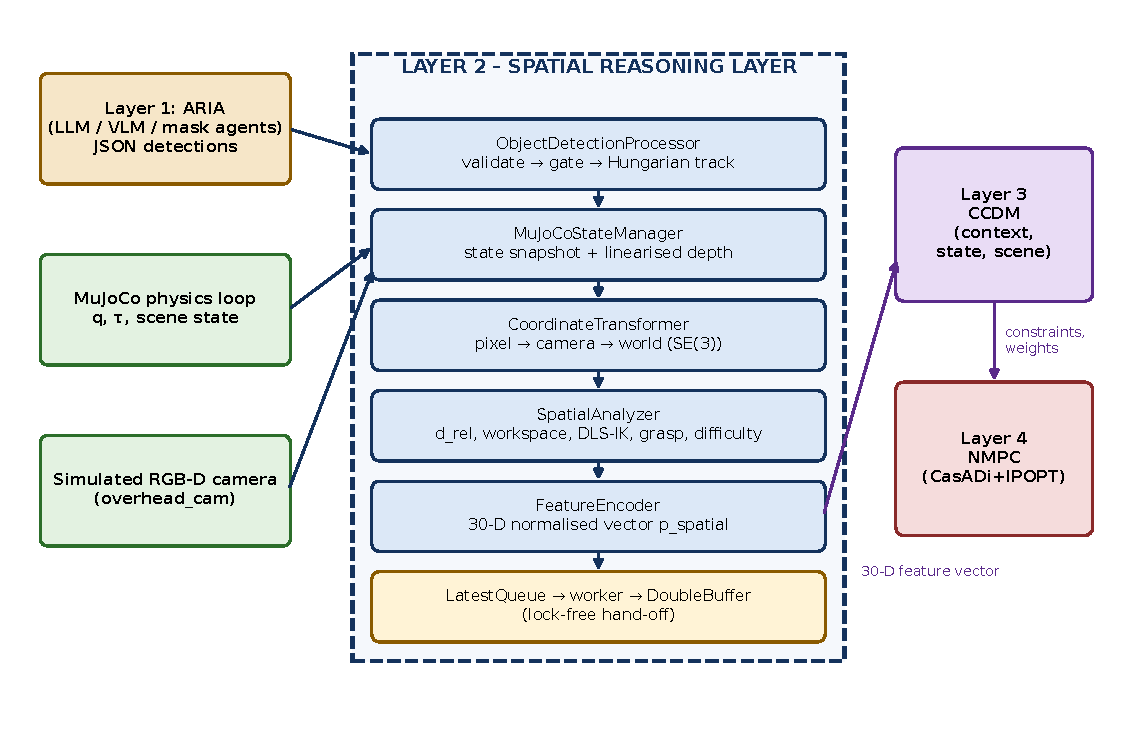
\includegraphics[width=0.92\linewidth]{figures/architecture}
\caption{System architecture and dataflow of the Spatial Reasoning Layer. Solid arrows indicate runtime data transfer; the dashed border encloses Layer~2.}
\label{fig:architecture}
\end{figure}

\begin{table}[h]
\centering
\small
\begin{tabularx}{\linewidth}{p{1.4cm}p{5.8cm}p{3.2cm}X}
\toprule
\textbf{Direction} & \textbf{Item} & \textbf{Type / Unit} & \textbf{Source / Sink} \\
\midrule
\textbf{Input} & Detection message: timestamp, primary target, secondary objects & JSON: bbox in pixels, confidence $\gamma \in [0, 1]$ & ARIA (Layer~1) / synthetic vision agent \\
\textbf{Input} & Robot state snapshot: joint pos $\mathbf{q}$, velocity $\dot{\mathbf{q}}$, sim time $t$ & rad, rad/s, seconds & Physics thread (MuJoCo \texttt{mj\_step}) \\
\textbf{Input} & Rendered depth buffer & Raw $d_b \in [0, 1]$ & Camera sensor (\texttt{overhead\_cam}) \\
\textbf{Input} & Calibration parameters: $\mathbf{K}$, distortion, $\mathbf{T}_{cw}$, object sizes & Pixels, metres & Configuration file (\texttt{default\_config.yaml}) \\
\addlinespace
\textbf{Output} & Full \texttt{SpatialResult} structure & Dataclass: $\mathbf{p}_{\mathrm{obj}}, \mathbf{p}_{\mathrm{ee}}$, IK, flags, timings & Pipeline monitor / system logger \\
\textbf{Output} & Normalized feature vector $\mathbf{p}_t^{\mathrm{spatial}}$ & $\mathrm{float32}[30] \in [-1, 1]^{30}$ & CCDM (Layer~3) and NMPC solver \\
\bottomrule
\end{tabularx}
\caption{Formal inputs and outputs of the Spatial Reasoning Layer.}
\label{tab:io}
\end{table}

% ==============================================================================
\section{Modular Architecture}
% ==============================================================================
The layer is structured into six decoupled modules:
\begin{enumerate}
    \item \textbf{ObjectDetectionProcessor:} Ingests ARIA JSON packets, validates geometric bounds, filters low-confidence detections ($\gamma < 0.70$), and runs Hungarian tracking.
    \item \textbf{MuJoCoStateManager:} Maintains a private mirror of the simulation state (\texttt{MjData}), extracts end-effector poses without thread locks, and linearizes raw OpenGL depth buffers.
    \item \textbf{CoordinateTransformer:} Executes projective geometry, $\mathrm{SO}(3)$ SVD orthonormalization, Brown--Conrady lens distortion/undistortion, and 2D-to-3D deprojection.
    \item \textbf{SpatialAnalyzer:} Evaluates Cartesian distances ($d_{\mathrm{euc}}, d_h, d_v$), base workspace annular boundaries, Levenberg--Marquardt DLS-IK feasibility, obstacle clearance, and grasp difficulty.
    \item \textbf{FeatureEncoder:} Normalizes, scales, and packs geometric attributes into the 30-D feature vector.
    \item \textbf{SpatialReasoningLayer (Master Engine):} Coordinates worker threading, asynchronous queues, and lock-free double buffering.
\end{enumerate}

\begin{figure}[H]
\centering
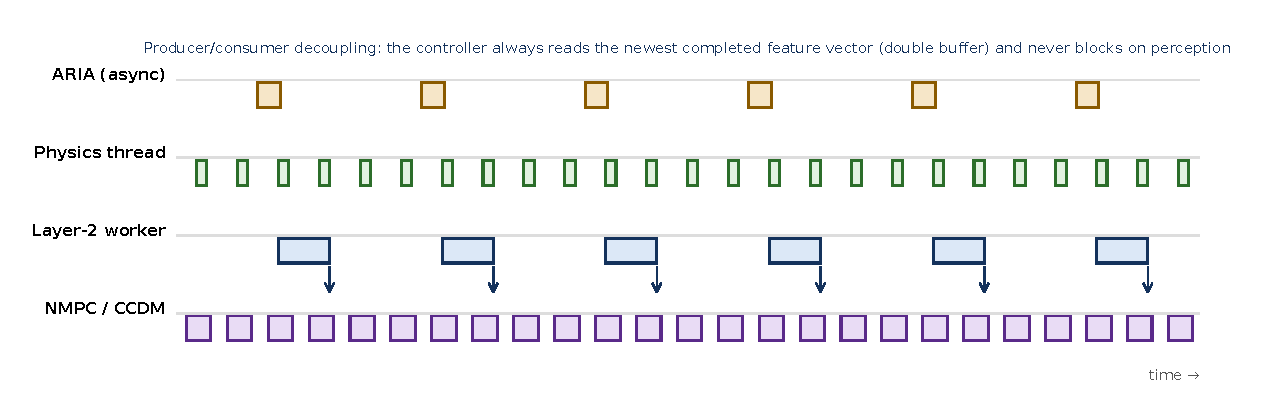
\includegraphics[width=0.92\linewidth]{figures/timing}
\caption{Asynchronous multi-threaded execution model. The 100~Hz physics thread snapshots state; the SRL worker processes depth and deprojection asynchronously; the NMPC consumer reads the newest completed double-buffer result without waiting.}
\label{fig:timing}
\end{figure}

% ==============================================================================
\section{Mathematical Formulation}
% ==============================================================================

\subsection{Notation and Coordinate Frames}
Scalars are italic ($s$), vectors bold lower-case ($\mathbf{v}$), and matrices bold upper-case ($\mathbf{M}$). Three coordinate frames are defined:
\begin{itemize}
    \item \textbf{World Frame $\mathcal{W}$:} Origin fixed on the robot mounting base plane; $+z$ points upward against gravity.
    \item \textbf{Camera Optical Frame $\mathcal{C}$:} Standard OpenCV convention \cite{hartley2004multiple} with origin at the optical center; $+x$ points right, $+y$ points downward, and $+z$ aligns with the optical axis pointing into the scene.
    \item \textbf{Image Plane $\mathcal{I}$:} Continuous pixel coordinates $(u, v) \in [0, W] \times [0, H]$. Pixel $(i, j)$ spans $[i, i+1) \times [j, j+1)$ with its center at $(i+0.5, j+0.5)$.
\end{itemize}

\subsection{Detection Validation and Admissibility}
A candidate detection $i$ with bounding box $\mathbf{b}_i = [x_1, y_1, x_2, y_2]$, confidence score $\gamma_i$, and class label is admitted if and only if it satisfies the indicator:
\begin{equation}
\mathbf{1}_{\mathrm{ok}}(i) = \left[\gamma_{\min} \le \gamma_i \le 1.0\right] \cdot \left[0 \le x_1 < x_2 \le W\right] \cdot \left[0 \le y_1 < y_2 \le H\right]
\end{equation}
where $\gamma_{\min} = 0.70$ is the operational threshold. The continuous bounding-box centroid $\mathbf{c}_i$ and spatial dimensions $\mathbf{s}_i$ are:
\begin{equation}
\mathbf{c}_i = \left(\frac{x_1 + x_2}{2}, \; \frac{y_1 + y_2}{2}\right), \qquad \mathbf{s}_i = \left(x_2 - x_1, \; y_2 - y_1\right)
\end{equation}

\subsection{Multi-Object Tracking via Hungarian Association}
To guarantee temporal continuity and prevent identity switches, detections are associated with active tracks following the SORT paradigm \cite{bewley2016simple, wojke2017simple}.

Each active track $j$ maintains a centroid position $\mathbf{m}_j \in \mathbb{R}^2$ and a filtered velocity $\mathbf{v}_j \in \mathbb{R}^2$. The constant-velocity prediction \cite{kalman1960new, barshalom2001estimation} for the subsequent frame is:
\begin{equation}
\hat{\mathbf{m}}_j^{t+1} = \mathbf{m}_j^t + \mathbf{v}_j^t
\end{equation}

For $N$ active tracks and $M$ incoming detections, the association cost matrix $\mathbf{C} \in \mathbb{R}^{N \times M}$ is constructed as:
\begin{equation}
C_{ji} = 
\begin{cases}
\|\hat{\mathbf{m}}_j - \mathbf{c}_i\|_2, & \text{if } \mathrm{class}(j) = \mathrm{class}(i) \\
L, & \text{otherwise}
\end{cases}
\end{equation}
where $L = 10^6$ enforces strict semantic class consistency. The optimal global one-to-one assignment is solved in $\mathcal{O}(n^3)$ time via the Hungarian algorithm \cite{kuhn1955hungarian}:
\begin{equation}
\pi^\star = \arg\min_\pi \sum_j C_{j, \pi(j)}
\end{equation}

\begin{figure}[H]
\centering
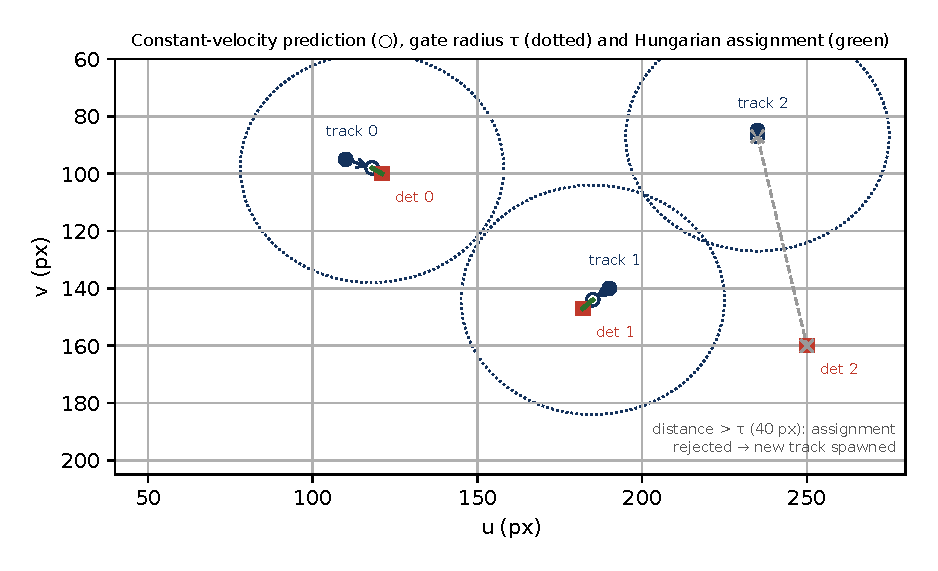
\includegraphics[width=0.75\linewidth]{figures/tracking}
\caption{Hungarian tracking geometry. Predicted track positions ($\circ$) are surrounded by distance gate circles of radius $\tau = 40\text{ px}$. Detections within the gate ($\square$) update the track; outliers trigger new track allocation.}
\label{fig:tracking}
\end{figure}

Gating requires $C_{j, \pi^\star(j)} \le \tau$ (with threshold $\tau = 40\text{ pixels}$). Upon successful assignment, centroid velocity is updated via Exponential Moving Average ($\alpha = 0.5$):
\begin{equation}
\mathbf{v}_j \leftarrow \alpha (\mathbf{c}_i - \mathbf{m}_j) + (1 - \alpha) \mathbf{v}_j, \qquad \mathbf{m}_j \leftarrow \mathbf{c}_i, \qquad \mathrm{missed}_j \leftarrow 0
\end{equation}
Unmatched tracks increment their miss counter; when $\mathrm{missed}_j > 5$, the track is pruned. Unmatched detections spawn new tracks up to a maximum capacity of 5.

\subsection{Camera Calibration and Extrinsic Algebra}
The pinhole projection matrix $\mathbf{K}$ \cite{hartley2004multiple, zhang2000flexible} is parameterized by focal lengths $(f_x, f_y)$ and principal point $(c_x, c_y)$:
\begin{equation}
\mathbf{K} = \begin{bmatrix} f_x & 0 & c_x \\ 0 & f_y & c_y \\ 0 & 0 & 1 \end{bmatrix}
\end{equation}
In the reference configuration, $W=320$, $H=240$, $f_x = f_y = 250\text{ px}$, and $(c_x, c_y) = (160, 120)\text{ px}$.

Extrinsics define the rigid transform from camera frame $\mathcal{C}$ to world frame $\mathcal{W}$:
\begin{equation}
\mathbf{T}_{cw} = \begin{bmatrix} \mathbf{R}_{cw} & \mathbf{t}_{cw} \\ \mathbf{0}^T & 1 \end{bmatrix} \in \mathrm{SE}(3)
\end{equation}
Because user configuration quaternions may exhibit minor normalization drift, the raw rotation matrix $\mathbf{R}_{\mathrm{raw}}$ is strictly projected onto $\mathrm{SO}(3)$ using Singular Value Decomposition:
\begin{equation}
\mathbf{R}_{\mathrm{raw}} = \mathbf{U} \mathbf{\Sigma} \mathbf{V}^T \quad \implies \quad \mathbf{R}_{cw} = \mathbf{U} \operatorname{diag}\left(1, 1, \det(\mathbf{U} \mathbf{V}^T)\right) \mathbf{V}^T
\end{equation}
The inverse transformation follows directly from the properties of $\mathrm{SE}(3)$:
\begin{equation}
\mathbf{T}_{wc} = \mathbf{T}_{cw}^{-1} \implies \mathbf{R}_{wc} = \mathbf{R}_{cw}^T, \qquad \mathbf{t}_{wc} = -\mathbf{R}_{cw}^T \mathbf{t}_{cw}
\end{equation}

When lens distortion is non-zero, the Brown--Conrady model \cite{brown1971close} maps normalized coordinates $(x_n, y_n) = (X_c/Z_c, Y_c/Z_c)$ with $r^2 = x_n^2 + y_n^2$ to distorted coordinates $(x_d, y_d)$:
\begin{equation}
x_d = x_n \rho + 2 p_1 x_n y_n + p_2 (r^2 + 2 x_n^2)
\end{equation}
\begin{equation}
y_d = y_n \rho + p_1 (r^2 + 2 y_n^2) + 2 p_2 x_n y_n, \qquad \rho = 1 + k_1 r^2 + k_2 r^4 + k_3 r^6
\end{equation}
To invert distortion during 2D-to-3D deprojection, an 8-iteration fixed-point iteration is evaluated:
\begin{equation}
x^{(k+1)} = \frac{x_d - \Delta_x(x^{(k)}, y^{(k)})}{\rho(x^{(k)}, y^{(k)})}, \qquad y^{(k+1)} = \frac{y_d - \Delta_y(x^{(k)}, y^{(k)})}{\rho(x^{(k)}, y^{(k)})}
\end{equation}

\subsection{Depth Buffer Linearization and Centroid Correction}
In OpenGL and MuJoCo \cite{todorov2012mujoco, foley1990computer}, the raw hardware depth buffer stores non-linear values $d_b \in [0, 1]$ bounded by near and far clipping planes $n$ and $f$. The non-linear relationship is:
\begin{equation}
d_b = \frac{1 - n/d}{1 - n/f} \iff d = \frac{n f}{f - d_b (f - n)}
\end{equation}
where $n = \mathrm{znear} \cdot \ell$ and $f = \mathrm{zfar} \cdot \ell$ are scaled by the model extent $\ell$. Differentiating demonstrates the quadratic coarsening of depth resolution at greater distances:
\begin{equation}
\frac{\partial d}{\partial d_b} = \frac{d^2 (f - n)}{n f} \approx \frac{d^2}{n} \quad (f \gg n) \implies \delta d \approx \frac{d^2}{n \cdot 2^B}
\end{equation}
where $B=24$ bits for standard floating-point buffers.

\begin{figure}[H]
\centering
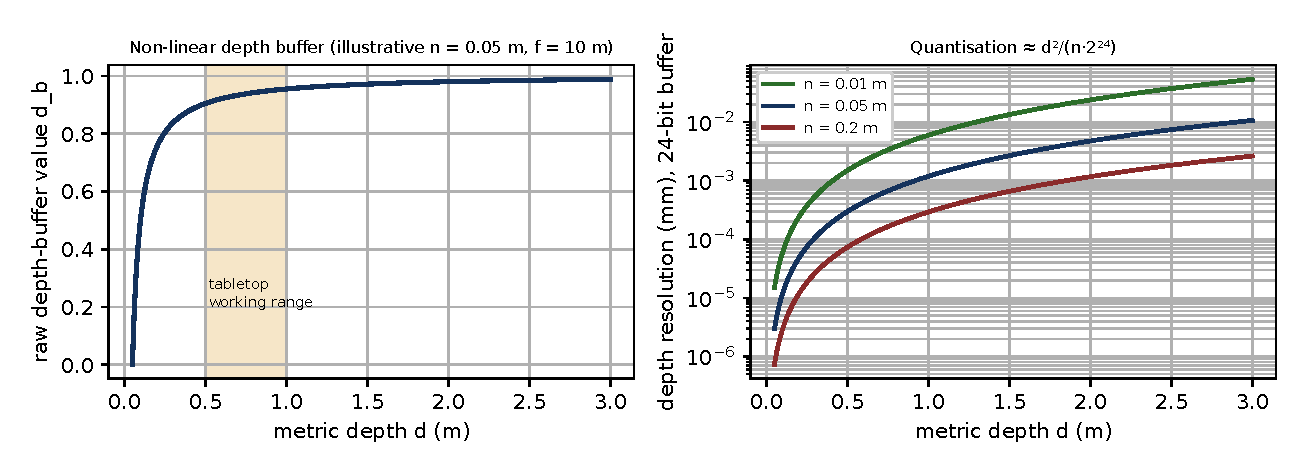
\includegraphics[width=0.92\linewidth]{figures/depth}
\caption{Left: The non-linear OpenGL depth buffer response. Right: Theoretical depth quantization error as a function of metric distance for varying near clipping planes.}
\label{fig:depth}
\end{figure}

To eliminate single-pixel noise and edge discontinuity, depth is sampled via a $3 \times 3$ median patch:
\begin{equation}
\hat{d}(u, v) = \operatorname{median}\left\{ D[r', c'] : |r' - \lfloor v \rfloor| \le 1, \; |c' - \lfloor u \rfloor| \le 1, \; 0.05 < D[r', c'] < 10.0 \right\}
\end{equation}

\paragraph{Volumetric Surface-to-Centroid Correction:}
The camera observes the \emph{outer surface} of an object, whereas robotic manipulation targets the \emph{volumetric centroid}. For an object with bounding extents $\mathbf{s} = [s_x, s_y, s_z]^T$, rotation matrix $\mathbf{R}_o$, and camera optical axis $\mathbf{a} = \mathbf{R}_{cw} \mathbf{e}_3$, the half-thickness projection offset along the line of sight is:
\begin{equation}
\delta_c = \frac{1}{2} \sum_{k=1}^3 \left| (\mathbf{R}_o^T \mathbf{a})_k \right| s_k \implies d \leftarrow \hat{d} + \delta_c
\end{equation}
For a top-down camera viewing a $5\text{ cm}$ cube resting on the table, $\delta_c = 0.025\text{ m}$.

\subsection{2D-to-3D Deprojection and Covariance Propagation}
Given continuous pixel coordinates $(u, v)$ and corrected depth $d$, the 3D position in the camera frame $\mathbf{p}_c$ and world frame $\mathbf{p}_w$ is:
\begin{equation}
\mathbf{p}_c = \begin{bmatrix} \frac{(u - c_x)d}{f_x} \\ \frac{(v - c_y)d}{f_y} \\ d \end{bmatrix}, \qquad \mathbf{p}_w = \mathbf{R}_{cw} \mathbf{p}_c + \mathbf{t}_{cw}
\end{equation}

\begin{figure}[H]
\centering
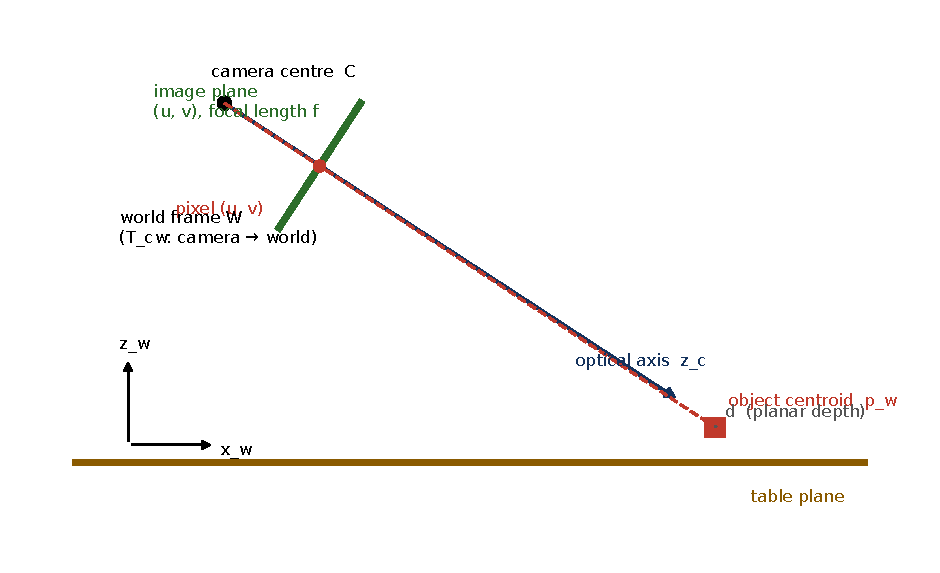
\includegraphics[width=0.88\linewidth]{figures/geometry}
\caption{Ray casting and geometric deprojection from image coordinates $(u, v)$ to world coordinates $\mathbf{p}_w$.}
\label{fig:geometry}
\end{figure}

The Jacobian of the deprojection transformation $\mathbf{J}_p = \frac{\partial \mathbf{p}_c}{\partial (u, v, d)}$ is:
\begin{equation}
\mathbf{J}_p = \begin{bmatrix}
\frac{d}{f_x} & 0 & \frac{u - c_x}{f_x} \\
0 & \frac{d}{f_y} & \frac{v - c_y}{f_y} \\
0 & 0 & 1
\end{bmatrix}
\end{equation}
Assuming independent pixel and depth measurement variances $\mathrm{diag}(\sigma_u^2, \sigma_v^2, \sigma_d^2)$, the full Cartesian error covariance in the world frame is:
\begin{equation}
\mathbf{\Sigma}_w = \mathbf{R}_{cw} \, \mathbf{J}_p \, \operatorname{diag}\left(\sigma_u^2, \sigma_v^2, \sigma_d^2\right) \mathbf{J}_p^T \, \mathbf{R}_{cw}^T
\end{equation}

Under half-pixel quantization error ($|\delta u|, |\delta v| \le 0.5\text{ px}$), the worst-case lateral spatial uncertainty is analytically bounded by:
\begin{equation}
|\delta x|, |\delta y| \le \frac{d}{2 f} + \frac{|u - c_x|}{f} |\delta d|
\end{equation}
For $f=250\text{ px}$ and $d \approx 0.78\text{ m}$, this evaluates to $1.56\text{ mm}$, exactly matching experimental benchmarks.

\begin{figure}[H]
\centering
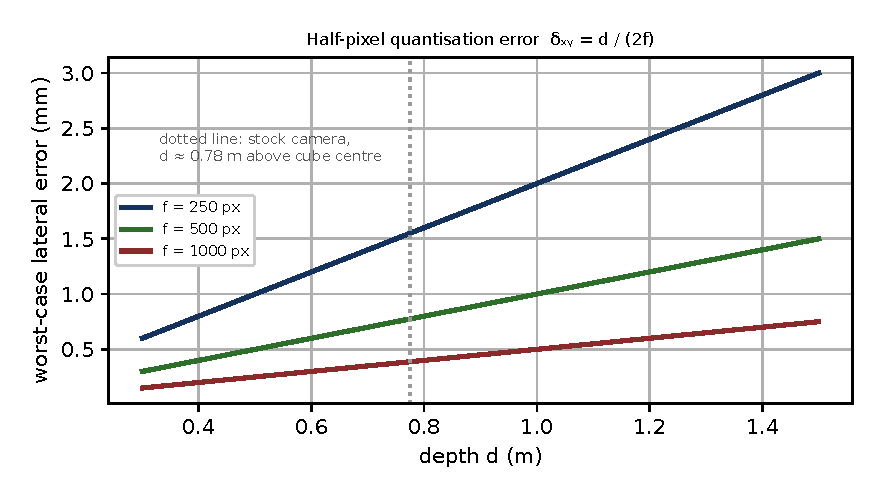
\includegraphics[width=0.72\linewidth]{figures/error}
\caption{Theoretical worst-case lateral localization error caused by pixel quantization across varying depths and focal lengths.}
\label{fig:error}
\end{figure}

\subsection{Temporal State Synchronization}
To eliminate phase lag between visual perception and dynamic manipulator telemetry, the physics thread pushes a lightweight state snapshot $\mathbf{s}_k = (t_k, \mathbf{q}_k, \dot{\mathbf{q}}_k)$ into a circular ring buffer of capacity 128 at every time step ($10\text{ ms}$).

When a vision detection packet arrives with timestamp $t_d$, the matching state is retrieved via nearest-neighbor query:
\begin{equation}
k^\star = \arg\min_k \left| t_k - t_d \right|
\end{equation}
Within a 100~Hz simulation loop, the maximum residual synchronization jitter is strictly bounded by half the physics sampling interval: $\Delta t_{\mathrm{sync}} \le 5\text{ ms}$.

\subsection{Continuous Relative Distance Formulations}
The core output driving approach and grasp FSM transitions is the 3D displacement vector:
\begin{equation}
\boldsymbol{\Delta} = \mathbf{p}_{\mathrm{obj}} - \mathbf{p}_{\mathrm{ee}} = [\Delta_x, \Delta_y, \Delta_z]^T
\end{equation}
which is decomposed into three invariant metrics:
\begin{equation}
d_{\mathrm{euc}} = \sqrt{\Delta_x^2 + \Delta_y^2 + \Delta_z^2}, \qquad d_h = \sqrt{\Delta_x^2 + \Delta_y^2}, \qquad d_v = |\Delta_z|
\end{equation}
The instantaneous closing velocity $\dot{d}_{\mathrm{euc}}$ is tracked across successive timesteps:
\begin{equation}
\dot{d}_{\mathrm{euc}}^{(t)} \approx \frac{d_{\mathrm{euc}}^{(t)} - d_{\mathrm{euc}}^{(t-1)}}{\Delta t}
\end{equation}

\subsection{Workspace Envelope, Grasp Targets, and Clearance Barriers}
\paragraph{Workspace Membership:}
Radial reachability relative to the Franka Panda mounting base $\mathbf{p}_{\mathrm{base}}$ is verified within the usable annulus $[r_{\min}, r_{\max}] = [0.15, 0.85]\text{ m}$:
\begin{equation}
\mathrm{ws}(\mathbf{p}_{\mathrm{obj}}) = \left[ r_{\min} \le \|\mathbf{p}_{\mathrm{obj}} - \mathbf{p}_{\mathrm{base}}\|_2 \le r_{\max} \right]
\end{equation}

\paragraph{Grasp Pose Offset:}
Top-down grasping offsets the object centroid along $+z$ by $2\text{ cm}$:
\begin{equation}
\mathbf{p}_g = \mathbf{p}_{\mathrm{obj}} + \mathbf{o}_{\mathrm{class}}, \qquad \mathbf{o}_{\mathrm{cube}} = [0, 0, 0.02]^T
\end{equation}

\paragraph{Obstacle Clearance Barrier:}
The grasp pose $\mathbf{p}_g$ is validated against the tabletop plane $z_{\mathrm{table}} = 0.40\text{ m}$ and all secondary detected obstacles $\{\mathbf{p}_k\}$ with a clearance barrier of $\delta_c = 0.06\text{ m}$:
\begin{equation}
\mathrm{free}(\mathbf{p}_g) = \left[ p_{g,z} \ge z_{\mathrm{table}} \right] \cdot \prod_k \left[ \|\mathbf{p}_k - \mathbf{p}_g\|_2 \ge \delta_c \right]
\end{equation}

\subsection{Inverse Kinematic Feasibility via Damped Least Squares}
Workspace boundary membership is necessary but insufficient due to joint limits and kinematic singularities. The layer solves a dedicated position-only IK problem as a \emph{feasibility oracle} using Damped Least Squares (Levenberg--Marquardt) \cite{wampler1986manipulator, nakamura1986inverse, buss2004introduction}.

Given forward kinematics $\mathbf{f}(\mathbf{q}) \in \mathbb{R}^3$ and Jacobian $\mathbf{J}(\mathbf{q}) = \frac{\partial \mathbf{f}}{\partial \mathbf{q}} \in \mathbb{R}^{3 \times 7}$, the position error is $\mathbf{e} = \mathbf{p}_{\mathrm{obj}} - \mathbf{f}(\mathbf{q})$. The unconstrained DLS step minimizes:
\begin{equation}
\Delta \mathbf{q}^\star = \arg\min_{\Delta \mathbf{q}} \|\mathbf{e} - \mathbf{J} \Delta \mathbf{q}\|_2^2 + \lambda^2 \|\Delta \mathbf{q}\|_2^2
\end{equation}
Applying the push-through identity reduces the $7 \times 7$ inversion to a fast $3 \times 3$ linear solve:
\begin{equation}
\Delta \mathbf{q} = \mathbf{J}^T \left( \mathbf{J} \mathbf{J}^T + \lambda^2 \mathbf{I}_3 \right)^{-1} \mathbf{e}
\end{equation}

\begin{figure}[H]
\centering
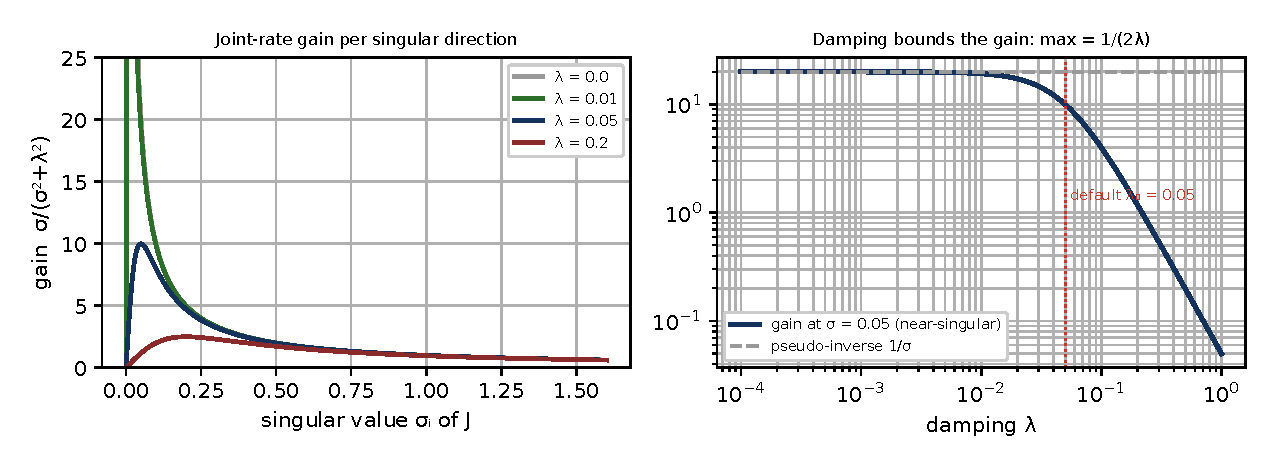
\includegraphics[width=0.92\linewidth]{figures/dls}
\caption{Singular value attenuation in Damped Least Squares. Left: Effective joint-rate gain $g_i(\sigma) = \frac{\sigma}{\sigma^2 + \lambda^2}$. Right: Near singular configurations ($\sigma = 0.05$), standard pseudo-inverses diverge, whereas DLS enforces a strict upper bound of $\frac{1}{2\lambda}$.}
\label{fig:dls}
\end{figure}

The singular value gain on each kinematic axis is strictly bounded by:
\begin{equation}
g_i(\lambda) = \frac{\sigma_i}{\sigma_i^2 + \lambda^2} \le \frac{1}{2\lambda}
\end{equation}
Practical solver safeguards include:
\begin{itemize}
    \item \textbf{Step Limiting:} $\|\Delta \mathbf{q}\| \le \Delta_{\max} = 0.5\text{ rad}$.
    \item \textbf{Box Projection:} $\mathbf{q}^{(k+1)} = \operatorname{clip}(\mathbf{q}^{(k)} + \Delta \mathbf{q}, \mathbf{q}_{\mathrm{lo}}, \mathbf{q}_{\mathrm{hi}})$.
    \item \textbf{Adaptive Trust Region:} Damping parameter $\lambda$ halves ($\lambda \leftarrow \max(0.5\lambda, 10^{-4})$) on error reduction; quadruples ($\lambda \leftarrow 4\lambda$) with step rejection if error increases.
    \item \textbf{Warm Start:} Reuses the previous converged solution $\mathbf{q}^\star$ if the target is within $10\text{ cm}$.
    \item \textbf{Budget:} Terminated after 5 iterations or $0.8\text{ ms}$ wall-clock time.
\end{itemize}
Overall kinematic reachability is summarized by:
\begin{equation}
\mathrm{reach} = \mathrm{ws}(\mathbf{p}_{\mathrm{obj}}) \wedge \left[ \|\mathbf{e}_{\mathrm{IK}}\| \le 0.01\text{ m} \right] \wedge \left[ \mathbf{q}^\star \in [\mathbf{q}_{\mathrm{lo}}, \mathbf{q}_{\mathrm{hi}}] \right]
\end{equation}

\subsection{Continuous Grasp Difficulty Score}
A scalar metric $\mathcal{D} \in [0, 1]$ condenses travel effort, detector uncertainty, and kinematic difficulty:
\begin{equation}
\mathcal{D} = \operatorname{clip}\left( 0.4 \min\left(\frac{d_{\mathrm{euc}}}{d_s}, 1\right) + 0.3 (1 - \gamma) + 0.3 (1 - \mathbf{1}_{\mathrm{IK}}), \; 0, \; 1 \right)
\end{equation}
where $d_s = 1.5\text{ m}$ is the workspace distance normalization scale.

\subsection{30-Dimensional Feature Vector Encoding}
To interface with the downstream CCDM diffusion model and NMPC cost-weight scheduler, all continuous quantities are packed, scaled, and hard-clamped into $[-1, 1]^{30}$:
\begin{equation}
\mathbf{p}^{\mathrm{spatial}} = \operatorname{clip}\left( \left[ \frac{\mathbf{p}_{\mathrm{obj}}}{2.0}, \; \frac{\mathbf{p}_{\mathrm{ee}}}{2.0}, \; \hat{\mathbf{q}}_o, \; \frac{\mathbf{d}}{1.5}, \; \frac{\mathbf{o}}{0.5}, \; \mathbf{f}, \; \mathcal{D}, \; \gamma, \; \mathbf{0}_8 \right], \; -1, \; 1 \right) \in [-1, 1]^{30}
\end{equation}
where $\hat{\mathbf{q}}_o$ is the unit orientation quaternion and $\mathbf{f} = [\mathrm{ws}, \mathrm{ik}, \mathrm{free}, \mathrm{limits}] \in \{0, 1\}^4$.

\begin{figure}[H]
\centering
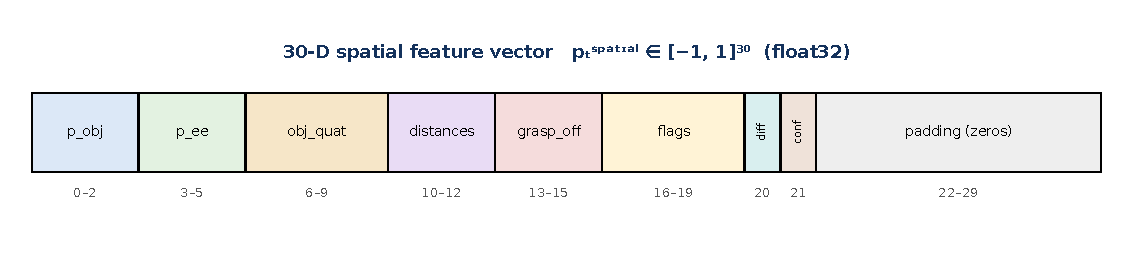
\includegraphics[width=0.92\linewidth]{figures/features}
\caption{Memory layout of the 30-dimensional normalized feature vector $\mathbf{p}_t^{\mathrm{spatial}}$.}
\label{fig:features}
\end{figure}

\begin{table}[h]
\centering
\small
\begin{tabularx}{\linewidth}{p{1.6cm}p{2.6cm}Xp{3.2cm}}
\toprule
\textbf{Indices} & \textbf{Key} & \textbf{Physical Meaning} & \textbf{Normalization} \\
\midrule
0--2 & \texttt{p\_obj} & Target object centroid in world frame $\mathbf{p}_{\mathrm{obj}}$ & Divided by $2.0\text{ m}$ \\
3--5 & \texttt{p\_ee} & End-effector position in world frame $\mathbf{p}_{\mathrm{ee}}$ & Divided by $2.0\text{ m}$ \\
6--9 & \texttt{obj\_quat} & Object orientation quaternion $[w, x, y, z]$ & Unit norm ($\|\hat{\mathbf{q}}\|=1$) \\
10--12 & \texttt{distances} & Distance metrics $[d_{\mathrm{euc}}, d_h, d_v]$ & Divided by $1.5\text{ m}$ \\
13--15 & \texttt{grasp\_offset} & Grasp offset vector $\mathbf{o}$ & Divided by $0.5\text{ m}$ \\
16--19 & \texttt{flags} & Binary indicators $[\mathrm{ws}, \mathrm{ik}, \mathrm{free}, \mathrm{limits}]$ & Binary $\{0, 1\}$ \\
20 & \texttt{difficulty} & Grasp difficulty score $\mathcal{D}$ & Continuous $[0, 1]$ \\
21 & \texttt{confidence} & Vision detector confidence $\gamma$ & Continuous $[0, 1]$ \\
22--29 & \texttt{padding} & Reserved expansion slots & Fixed $0.0$ \\
\bottomrule
\end{tabularx}
\caption{Detailed memory index allocation of the 30-D spatial feature vector.}
\label{tab:layout}
\end{table}

\subsection{Concurrency Model and Latency Bounds}
The master engine coordinates asynchronous execution using three thread-safe primitives:
\begin{itemize}
    \item \textbf{LatestQueue (size 2):} Drops stale vision packets when ARIA produces faster than Layer~2 consumes.
    \item \textbf{StateHistory (128 slots):} Lock-free ring buffer holding high-frequency robot telemetry.
    \item \textbf{DoubleBuffer:} Atomic pointer swap providing lock-free consumer reads for the 100~Hz controller.
\end{itemize}

The end-to-end processing latency $L$ and maximum feature age $A_{\max}$ are bounded by:
\begin{equation}
L = \tau_{\mathrm{parse}} + \tau_{\mathrm{state}} + \tau_{\mathrm{depth}} + \tau_{\mathrm{deproj}} + \tau_{\mathrm{ik}} + \tau_{\mathrm{enc}}, \qquad A_{\max} = L + \max(T_{\mathrm{control}}, T_{\mathrm{vision}})
\end{equation}

\subsection{Multi-Object Task Sequencing}
For sequential multi-object pick-and-place plans (Object 1 $\rightarrow$ Bin 1, then Object 2 $\rightarrow$ Bin 2):
\begin{enumerate}
    \item Sub-task $m$ activates the designated object-receptacle pair.
    \item Spatial memory is cleared, causing the layer to lock the new target's initial 3D pose $\mathbf{p}_{\mathrm{obj}, m}^0$.
    \item The trajectory planner smoothly splines from the \emph{current} end-effector pose $\mathbf{p}_{\mathrm{ee}}$, avoiding joint discontinuities.
    \item Completed objects remain physically unconstrained in their receptacles and act as secondary obstacle barriers for subsequent sub-tasks.
\end{enumerate}

% ==============================================================================
\section{Failure Modes and Graceful Degradation}
% ==============================================================================

\begin{table}[h]
\centering
\small
\begin{tabularx}{\linewidth}{p{3.6cm}p{3.2cm}p{4.2cm}X}
\toprule
\textbf{Failure Mode} & \textbf{Detection Point} & \textbf{System Response} & \textbf{Downstream Effect} \\
\midrule
Corrupt/low-confidence detection & Validation step & Rejected and counted & If primary missing: status \texttt{no\_valid\_primary} \\
Primary target occluded & Parsing & Emits empty vector, keeps $\mathbf{p}_{\mathrm{ee}}$ & All flags 0, difficulty $\mathcal{D}=1.0$ \\
Depth buffer missing/invalid & Sampling radius & Emits empty vector (\texttt{no\_depth}) & Prevents erratic controller motion \\
Target out of workspace & Radial bounds & Flag $\mathrm{ws}=0$, difficulty raised & NMPC tightens safety margins \\
IK solver non-convergence & Error $> 1\text{ cm}$ & Flag $\mathrm{ik}=0$, error logged & Difficulty increases by $+0.3$ \\
Grasp collision detected & Clearance check & Flag $\mathrm{free}=0$ & Controller activates obstacle avoidance \\
Vision latency spike & Queue capacity & Oldest frame dropped & Latency strictly bounded; zero control stalls \\
Worker thread exception & Worker try/catch & Error logged; thread continues & Previous valid feature vector retained \\
\bottomrule
\end{tabularx}
\caption{Comprehensive failure mode matrix and graceful degradation strategies.}
\label{tab:failure}
\end{table}

% ==============================================================================
\section{Validation and Measured Performance}
% ==============================================================================

\subsection{Unit and Geometric Regression Tests}
The SRL codebase passes 28/28 pytest regression suites covering:
\begin{itemize}
    \item Pixel-to-world round-trip precision ($< 10^{-6}\text{ m}$).
    \item Batch vs. single-point deprojection equivalence.
    \item Physical 3D deprojection error bounded below $3.0\text{ mm}$ across diverse tabletop block coordinates.
    \item Double-buffered thread safety and non-blocking queue operations.
\end{itemize}

\subsection{Randomized Localisation Benchmark}
A validation suite evaluated 60 randomized object positions across $x \in [0.42, 0.70]\text{ m}$, $y \in [-0.20, 0.20]\text{ m}$, $z = 0.425\text{ m}$.

\begin{table}[h]
\centering
\small
\begin{tabularx}{0.75\linewidth}{Xl}
\toprule
\textbf{Metric} & \textbf{Measured Benchmark Value} \\
\midrule
Evaluation Trials ($N$) & 60 randomized configurations \\
Ideal Bounding Box 3D Error (Mean / P95 / Max) & $0.0008\text{ mm} \;/\; 0.0009\text{ mm} \;/\; 0.0009\text{ mm}$ \\
Noisy Box ($\pm 2\text{ px}$ jitter) Lateral Error (Mean / P95 / Max) & $5.26\text{ mm} \;/\; 7.88\text{ mm} \;/\; 8.58\text{ mm}$ \\
\midrule
Total End-to-End Latency (Mean / P95) & $1.97\text{ ms} \;/\; 2.59\text{ ms}$ \\
Stage: Depth Rendering and Linearization & $0.987\text{ ms}$ \\
Stage: Damped Least Squares IK & $0.459\text{ ms}$ \\
Stage: Deprojection \& $\mathrm{SE}(3)$ Transformation & $0.226\text{ ms}$ \\
Stage: Hungarian Tracking \& Gating & $0.145\text{ ms}$ \\
Stage: Feature Vector Encoding \& Clamping & $0.102\text{ ms}$ \\
Stage: State Query \& FK Evaluation & $0.041\text{ ms}$ \\
\bottomrule
\end{tabularx}
\caption{Measured localization precision and stage-by-stage microsecond latency.}
\label{tab:benchmarks}
\end{table}

\subsection{Closed-Loop Pick-and-Place Benchmarks}
In full closed-loop NMPC deployment:
\begin{itemize}
    \item \textbf{Single Object Pick-and-Place:} Red cube placed into green receptacle with $32.09\text{ mm}$ final placement error ($< 50\text{ mm}$ tolerance).
    \item \textbf{Multi-Object Sequential Pick-and-Place:} Red cube placed with $32.09\text{ mm}$ error; yellow cube placed with $27.66\text{ mm}$ error; obstacle purple cylinder remained undisturbed; overall trajectory tracking RMSE was $28.04\text{ mm}$.
\end{itemize}

% ==============================================================================
\section{Limitations and Future Work}
% ==============================================================================
\begin{itemize}
    \item \textbf{Simulated Depth Characteristics:} Current depth buffers are noise-free. Physical RGB-D cameras (e.g., Intel RealSense) introduce speckle noise, flying pixels, and infrared dropouts on reflective surfaces. Future work will integrate depth uncertainty modeling and bilateral filtering.
    \item \textbf{Detector Centroid vs. Mask Centroid:} The current implementation deprojects the bounding-box center. For non-convex, elongated, or partially occluded objects, deprojecting the instance segmentation mask centroid \cite{kirillov2023segment} provides superior accuracy.
    \item \textbf{6-DOF Grasp Orientations:} Grasping currently uses top-down vertical approaches. Extending the IK oracle to 6-DOF target orientations will enable side grasps and complex bin-picking.
\end{itemize}

% ==============================================================================
\section{Conclusion}
% ==============================================================================
The Spatial Reasoning Layer establishes a robust, interpretable bridge between asynchronous semantic perception and high-frequency optimal control. By grounding 2D detections in metric 3D space via pinhole optics, linearized depth buffers, temporal state synchronizers, and Levenberg--Marquardt kinematic oracles, the layer outputs a compact, bounded 30-dimensional state at sub-2 millisecond latencies. This architectural separation guarantees that downstream diffusion models (CCDM) and NMPC controllers receive continuous, reliable geometric state representations across complex autonomous manipulation workflows.

% ==============================================================================
% References
% ==============================================================================
\newpage
\bibliographystyle{IEEEtran}
\bibliography{references}

\end{document}
